\documentclass{beamer}
%
% Choose how your presentation looks.
%
% For more themes, color themes and font themes, see:
% http://deic.uab.es/~iblanes/beamer_gallery/index_by_theme.html
%
\mode<presentation>
{
  \usetheme{default}      % or try Darmstadt, Madrid, Warsaw, ...
  \usecolortheme{default} % or try albatross, beaver, crane, ...
  \usefonttheme{default}  % or try serif, structurebold, ...
  \setbeamertemplate{navigation symbols}{}
  \setbeamertemplate{caption}[numbered]
} 

\usepackage[english]{babel}
\usepackage[utf8x]{inputenc}
\usepackage[font=small]{caption}
\graphicspath{ {./img/} }

\title[PR1/2 Demo]{PR1/2 Demo}
\author{Christian Permann}
\institute{Faculty of Computer Science, University of Vienna,\newline W\"ahringer Stra{\ss}e 29, 1090 Vienna}
\date{28.10.2018}

\begin{document}

\begin{frame}
  \titlepage
\end{frame}

% Uncomment these lines for an automatically generated outline.
%\begin{frame}{Outline}
%  \tableofcontents
%\end{frame}

\section{Introduction}

\begin{frame}{Milestones P1}

\begin{itemize}
  \item Create a basic visualization tool. (done)
  \item Define interface for data manipulation. (done)
  \item Be compatible with ELKI. (in progress)
  \item Allow data import. (CSV available)
  \item Create data generation logic. (ELKI generator available, in progress)
  \item Possibly plan for dim-reduction for visualization and implement it. (PCA, etc)

\end{itemize}

\vskip 1cm

\begin{block}{The existing tool}
The current iteration can visualize points, allows for generating points via the ELKI XML-based generator and was tested for performance with up to 300.000 points for a smooth experience.
\end{block}

\end{frame}

\begin{frame}{Milestones P2}

\begin{itemize}
\item Get to know ELKI. (in progress)
\item Enable running (ELKI) algorithms from the custom tool.
\item Properly save and display clustered data.
\item Enable defining presets and running multiple clusterings.
\item Allow for parameter space exploration within results.
\end{itemize}

\end{frame}

\section{Tool}

\begin{frame}{The Tool}

\centerline{Demo}

\end{frame}

\begin{frame}{The Tool - Data Generation Interface}

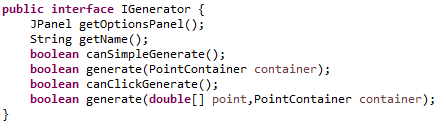
\includegraphics[width=\textwidth]{interface}
\captionof{figure}{The interface for data manipulation}

\end{frame}

\section{Clustervision}

\begin{frame}{Possible Improvements on Clustervision}

Clustervision ranks clustering results according to some quality measures but does not look further into the similarity between clusterings. Their ranking does think about not showing too similar clusterings at a high rank but the chosen similarity only looks at the labels, whereas it would be important to consider information like if two points, which were in the same cluster, are now in the same cluster as well. Clustering the cluster results with such a metric might be computationally expensive but may show more relevant differences in the results. Also defining a good distance metric for this difference seems non-trivial.

\end{frame}

\section{Data-sets}

\begin{frame}{Data-sets}
\begin{itemize}
\item real data-sets\cite{realdata}
\item well-known sets (benchmark sets)\cite{wellknown}
\item generated sets with different distributions

\end{itemize}
\end{frame}

\section{ELKI Algorithms}

\begin{frame}{ELKI Algorithms}
\begin{itemize}
\item DBSCAN: epsilon, minpts 
\item GeneralizedDBSCAN: coremodel, corepred, npred 
\item LSDBC: alpha, k(knn)
\item GriDBSCAN: epsilon, gridwidth, minpts
\item OPTICSHeap: epsilon, minpts
\item DeLiClu: minpts
\item FastOPTICS: (Random projection) index, minpts
\item KMeansLloyd: initializer, k, maxiter
\item many many more... \cite{clusterAlgorithms}

\end{itemize}

\end{frame}

\bibliography{citations}
\bibliographystyle{ieeetr}

\end{document}